\section{Dated verification and semi-analytic profile assessment}
\label{sec:autonomous-campaign}
The 19 October 2026 campaign extends the earlier evidence without replacing
its frozen records. Its questions are whether the implemented analyzer
handles specified changes of representation, whether a constructed solution
checks the original physical equations, and whether learning the remaining
profile is useful at matched accuracy. Exact structure is established before
approximation; neither a new general Lie theorem nor a learned first integral
is claimed.

\subsection{Geometric and source controls}
The consulted Olver volume is the 1986 first edition: Theorem 2.36,
printed p.~113, gives the prolongation formula, while Theorem 2.71,
printed p.~165, requires local solvability for the necessary infinitesimal
criterion \cite{olver}. These anchors do not refer to the second edition.
Oliveri's discussion of invariant graphs, restrictions on data and
one-dimensional subalgebras supplies complementary context
\cite{oliveri2026}. Figure~\ref{fig:autonomous-orbits} distinguishes a graph,
its group orbits and the quotient; their dimensions answer different questions.
The accompanying English account gives the chain-rule derivation, a fully
expanded heat-equation example, jet counting and local reconstruction.

\begin{figure}[htbp]
\centering
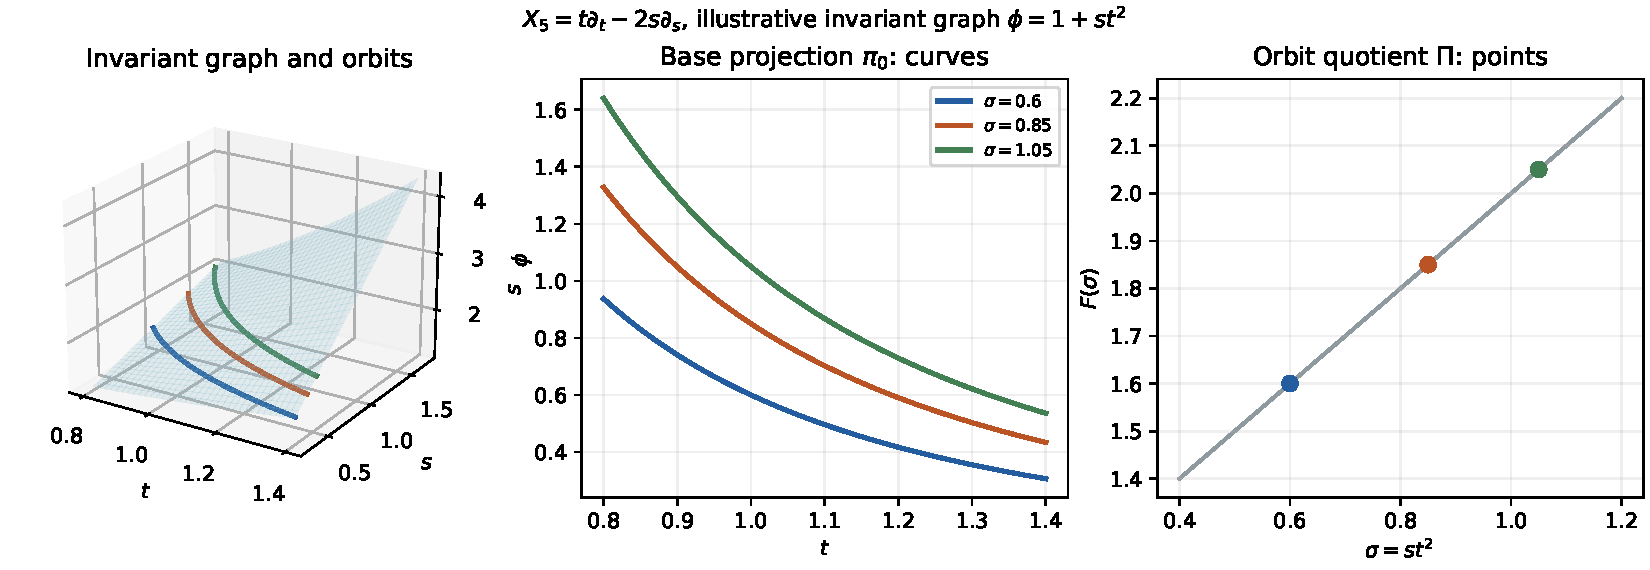
\includegraphics[width=\linewidth]{draft/figures/autonomous-orbit-geometry.pdf}
\caption{The action of $X_5=t\partial_t-2s\partial_s$ preserves
$\sigma=st^2$. The illustrative graph $\phi=1+st^2$ is invariant, but is
not asserted to solve SVE. Curves along the graph project to base orbits;
the quotient retains one coordinate per orbit. Graph invariance, quotient
rank and satisfaction of the PDE are distinct checks.}
\label{fig:autonomous-orbits}
\end{figure}

Arbitrary-function symmetries also need their defining differential
constraint: for the heat equation, $f(t,x)\partial_u$ is admitted when
$f_t-f_{xx}=0$, not for every smooth $f$. The arbitrary-function/Darboux
equivalence introduced as ``Theorem 1'' in the read preprint of
Gubbiotti, Levi and Scimiterna is explicitly conjectural
\cite{gubbiotti2015}. Bluman and de la Rosa's derivative-variable
construction retains integrability and a reconstruction constant
\cite{bluman2024}; it is distinct from merely reducing the number of
independent variables. These source distinctions prevent a large symmetry
family from being mistaken for general closed-form solvability.

\subsection{What the executable analyzer verified}
\label{sec:autonomous-analyzer}
The generic kernel constructs prolonged residuals and checks supplied
generators/charts. Its bounded differential-completion backend does not
solve arbitrary determining systems. The campaign exercised that existing
kernel through adapters, rather than replacing it with a table of known
generators. On a regular shell, the principal derivative was eliminated
before the candidate residual was tested. A negative candidate has an exact
nonzero admissible-jet witness; an unsupported computation is a separate
status. Noninteger powers were evaluated on the positive branch.

\begin{table}[htbp]\centering\small
\begin{tabularx}{\linewidth}{@{}l r X@{}}\toprule
Configuration family & Count & Change or check \\\midrule
Scalar exponent/parameter/model & 10 & $m=1,2,5/2,2.9,3,3.1$;
fixed dimensionless $\kappa$ versus $\beta$; printed versus material \\
Eulerian presentations & 3 & Primitive, conservative, invertible recombination \\
Coordinate/equation presentations & 2 & Constant coordinate rescaling; nonzero multiplier \\
Constitutive controls & 2 & Zero transport; fixed linear drag \\
Special checks & 12 & Mixed prolongations, arbitrary-function condition,
data/chart failures, input limits, parameter convention, coefficient
appendix, two obstructions, source Equation (27) \\\bottomrule
\end{tabularx}
\caption{The 29 configurations include 98 supplied-candidate occurrences:
77 exact acceptances and 21 exact rejections. Repeated occurrences across
presentations are not distinct discovered symmetries.}
\label{tab:autonomous-symbolic}
\end{table}

The repaired campaign passed 31 receipt checks in 39.60 seconds of
subprocess wall time, with 32.38 sampled CPU seconds and a largest
OS-reported working set of 72.80 MB. Each case had a 120-second and 8-GiB
limit; none timed out. Cold and warm timings are recorded separately.
Review exposed an empty-result acceptance path: an unsupported result with
no equations could satisfy a vacuous all-zero test. The adapter now checks
status, prerequisite checks and exact residual arity; four injected failure
cases are rejected. The initial receipts remain preserved, and the complete
rerun retained the 77/21 outcomes.

An independent implementation reconstructed all 118 coefficients of the
unrestricted point determining expansion and both obstruction witnesses
$3g\kappa$. Those checks alone do not complete the determining-system
integration. Separately, eight checks of the staged general-$m$ deductions
and sufficient residuals support the printed-model local classification
already proved in Section~\ref{sec:sve-repro}. Neither result classifies
the full Eulerian system or the advectively corrected scalar model.

\subsection{Independent original-system numerical experiment}
The exact member~\eqref{eq:autonomous-affine} was used at $g=1$,
$\beta=0.3$, $H_*=T_*=1$, $x_0=t_0=B_0=0$ on
$x\in[1,2]$, $t\in[1,1.3]$. A separate finite-volume solver evolves
$(h,hu,B)$ with Rusanov flux, a centered smooth bed-slope source and
SSPRK2; exact cell averages supply its initial and ghost data. This is an
original-PDE computation, separate from evolving the three-state ODE.
On the positive branch its primitive symbol is diagonally similar to a
symmetric irreducible tridiagonal matrix with off-diagonals
$\sqrt{gh}$ and $u\sqrt{g\beta}$. Thus its eigenvalues are real and
simple. The CFL bound $|u|+\sqrt{gh}+|u|\sqrt{g\beta}$ includes ghost
cells. This property does not prove convergence of the chosen discretization.

\begin{table}[htbp]\centering\small
\begin{tabular}{@{}rrrrr@{}}\toprule
Cells & $\|h-h_*\|_\infty$ & $\|u-u_*\|_\infty$
& $\|B-B_*\|_\infty$ & Solve time (s) \\\midrule
32 & $9.8545\,10^{-4}$ & $3.3329\,10^{-3}$ & $2.3342\,10^{-3}$ & 0.0197 \\
64 & $5.8097\,10^{-4}$ & $1.7332\,10^{-3}$ & $1.2025\,10^{-3}$ & 0.0407 \\
128 & $3.2591\,10^{-4}$ & $9.0156\,10^{-4}$ & $6.1377\,10^{-4}$ & 0.0846 \\\bottomrule
\end{tabular}
\caption{Final errors against exact cell-average fields; $u_*$ is the
ratio of exact discharge and depth averages. All three errors decrease.
The notation $*$ here denotes the exact reference, not a fitted parameter.}
\label{tab:autonomous-pde}
\end{table}

Accepted-step states remained positive and open-domain water/sediment
balances closed to roundoff when numerical boundary fluxes were included.
Three one-percent perturbations within the affine initial-data class were
also evolved; their DOP853/Radau reference discrepancy was below
$3.73\times10^{-13}$. They are restricted perturbation diagnostics.
Exact boundary traces at both ends are a consistency fixture, not a general
characteristic boundary solver. There is no wet/dry, shock, well-balanced,
arbitrary-data or measured-field validation claim.

\subsection{Two profile tasks and the learning protocol}
The first task uses the affine state $Y=(H,a,c)$; the second uses the
material common-scaling profile $Y=(F,P,C)$ with initial data
$(2,1/2,1/10)$, $g=1$, $\kappa=1/30$. Both core intervals are
$[1,7/5]$ at $m=3$. For the second task define
\[
 V=F-zP,\qquad
 L=-Fz^2+\frac{gF}{P^3}+\frac{gm\kappa zV^{m-1}}{P}.
\]
The independently checked normal form is
$F'=P$, $P'=C$,
$C'=-(L_z+P L_F+C L_P)C/L$, on $P,V>0$, $L\ne0$.
Its first integral $LC=I$ gives a separate two-state comparator with
the same $I=L(1,F_0,P_0)C_0$. The quotient and this order reduction
remain different operations. The fixed-$\kappa$ family uses the surviving
common scaling, not an invalid continuation of $X_5$.

Let $\xi=z-1$, $f_0=f(1,Y_0)$ and
$f_1=f_z(1,Y_0)+D_Yf(1,Y_0)f_0$. The three state representations are
\begin{align*}
 \widehat Y_{N0}&=Y_0+\xi N_\theta,\\
 \widehat Y_{K1}&=Y_0+\xi f_0+\xi^2N_\theta,\\
 \widehat Y_{H1}&=Y_0+\xi f_0+\tfrac12\xi^2 f_1+\xi^3N_\theta.
\end{align*}
The latter removes known Taylor coefficients before learning the remainder;
it does not learn the differential law or lower ODE order. All networks
have two width-16 tanh hidden layers in float64, 64 Gauss collocation
points, 700 Adam steps and a 500-evaluation L-BFGS budget. The loss is the
equally weighted first-order state defect. Original unnormalized residuals
and errors are evaluated independently on 1001 points. Each subprocess
has a 180-second/8-GiB bound on a CPU-only machine with two threads.

The frozen design has 12 N0/H1 runs (two tasks, seeds 17, 29, 43), two
K1 ablations (seed 17), and three conditional H2 models. H2 uses whole
profiles, with the following $(m,\eta)$ pairs:
\[
\begin{aligned}
\text{training: }&(2.9,-0.1),\ (3.1,-0.1),\ (3,0.1),\\
\text{validation: }&(3,0),\qquad
\text{test: }(2.95,-0.05),\ (3.05,-0.05).
\end{aligned}
\]
The initial data are
$Y_0=(2,1/2,(1+\eta)/10)$. The model/protocol hashes are frozen before
held-out evaluation. This tests interpolation within a small prescribed
family, not arbitrary-data generalization.

All gates must hold: maximum state error $\le10^{-5}$, raw first-order
and original residuals $\le10^{-4}$, initial mismatch $\le10^{-12}$,
and chart guards. For the scalar task the original residual uses actual
derivatives of $\widehat F$ through order three. Review additionally
checks its actual initial trace $(\widehat F,\widehat F',\widehat F'')$,
rather than equating independent state channels to that trace. This
evaluation-only addendum preserves the original failed outcomes.

\subsection{Measured outcomes and a derivative-compatibility diagnostic}
\begin{table}[htbp]\centering\small
\begin{tabular}{@{}lrrrr@{}}\toprule
Task/control & Reference discrepancy & C1 state error & C1 raw residual & C1 setup (s) \\\midrule
Affine & $3.64\,10^{-14}$ & $2.55\,10^{-15}$ & $2.33\,10^{-12}$ & 0.0103 \\
Material & $6.29\,10^{-14}$ & $1.02\,10^{-14}$ & $4.49\,10^{-6}$ & 0.0126 \\\bottomrule
\end{tabular}
\caption{DOP853/Radau cross-checks and degree-16 Chebyshev reuse (C1).
Setup includes reference integration; residuals differentiate the actual
polynomial. These are numerical controls, not rigorous enclosures.}
\label{tab:autonomous-classical}
\end{table}

Both single-profile classical controls pass. The maintained nonlinear
Chebyshev collocation is also checked separately. None of the 17 frozen
neural runs passes every gate: 0/12 core, 0/2 ablations and 0/3 conditional
models. Linear classical interpolation over the same three training
profiles also fails its held-out gates; those failures and fallback costs
are retained. The comparison therefore does not assume that every
nonlearned family surrogate succeeds. Solver choices and BVP restrictions
are checked against the installed SciPy 1.17.1 documentation
\cite{scipy1171ivp,scipy1171bvp}. No IVP is silently replaced by a BVP.

For independent channels define
$r_1=\widehat F'-\widehat P$ and $r_2=\widehat P'-\widehat C$.
Then the exact identities
\begin{equation}\label{eq:autonomous-compatibility}
 \widehat F''-\widehat C=r_2+r_1',\qquad
 \widehat F'''-\widehat C'=r_2'+r_1''
\end{equation}
show why small first-order defects alone do not control the strong scalar
residual. For example, seed-17 material N0 has state error
$7.24\times10^{-5}$, first-order defect $1.92\times10^{-3}$, but raw
scalar residual $1.58$; H1 has $1.75\times10^{-5}$,
$3.44\times10^{-4}$ and $0.232$, respectively. Neither passes.
The actual initial scalar traces also reject N0 and K1; H1's
equation-derived derivatives enforce those traces.

A separately frozen exploratory follow-up, motivated by this diagnostic,
uses one scalar network with $P,C$ obtained by differentiation:
$\widehat F=P_2(\xi)+\xi^3N_\theta$ or
$\widehat F=P_3(\xi)+\xi^4N_\theta$, where
$P_2=F_0+P_0\xi+C_0\xi^2/2$ and
$P_3=P_2+G(1,Y_0)\xi^3/6$, with $G=C'$ from the verified ODE.
Across six seeded runs the compatibility defects vanish by construction,
but state errors are $1.16\times10^{-5}$--$2.85\times10^{-5}$ and
raw scalar residuals $0.00515$--$0.0133$ on a separate 1201-point grid.
Thus 0/6 passes. Removing the representation defect did not solve the
bounded optimization problem, and this adaptive follow-up is exploratory.

All 23 runs produced recorded evaluations; 21 reached the full 500
L-BFGS evaluations. Completion is not optimizer convergence. Combined
campaign wall time was 284.02 seconds with largest sampled child RSS
361.17 MB. Saved weights, 29 profile evaluations, hashes and residuals
were replayed. Costs include setup, training, reference generation where
used, derivatives, verification and fallback. No matched-accuracy neural
break-even is established; fixed-profile cost curves are not a valid
substitute for H2's family comparison.

Derivative-norm tanh approximation theorems establish existence of
approximants under smoothness assumptions \cite{deryck2021tanh}; they do
not certify these widths, optimizer convergence or continuous residuals.
The benchmark/failure literature motivates multiple seeds and explicit
negative outcomes \cite{pinnacle2023v2,krishnapriyan2021}. Learning a
solution remainder for a fixed law is also distinct from learning a
component of a universal differential equation \cite{rackauckas2021}.
For the tested tasks the evidence favors classical solution/reuse.
No continuous learned-error certificate, general neural impossibility,
or selector trained from these few task records is inferred.
